\section{Problem  formulation}
\label{sec:problem}

Describe  your  problem  formulation,  any  data  processing  that  
will  beneeded, the performance measures that will be used and why, 
etc.

%\begin{figure*}[t]
%	\centering
%	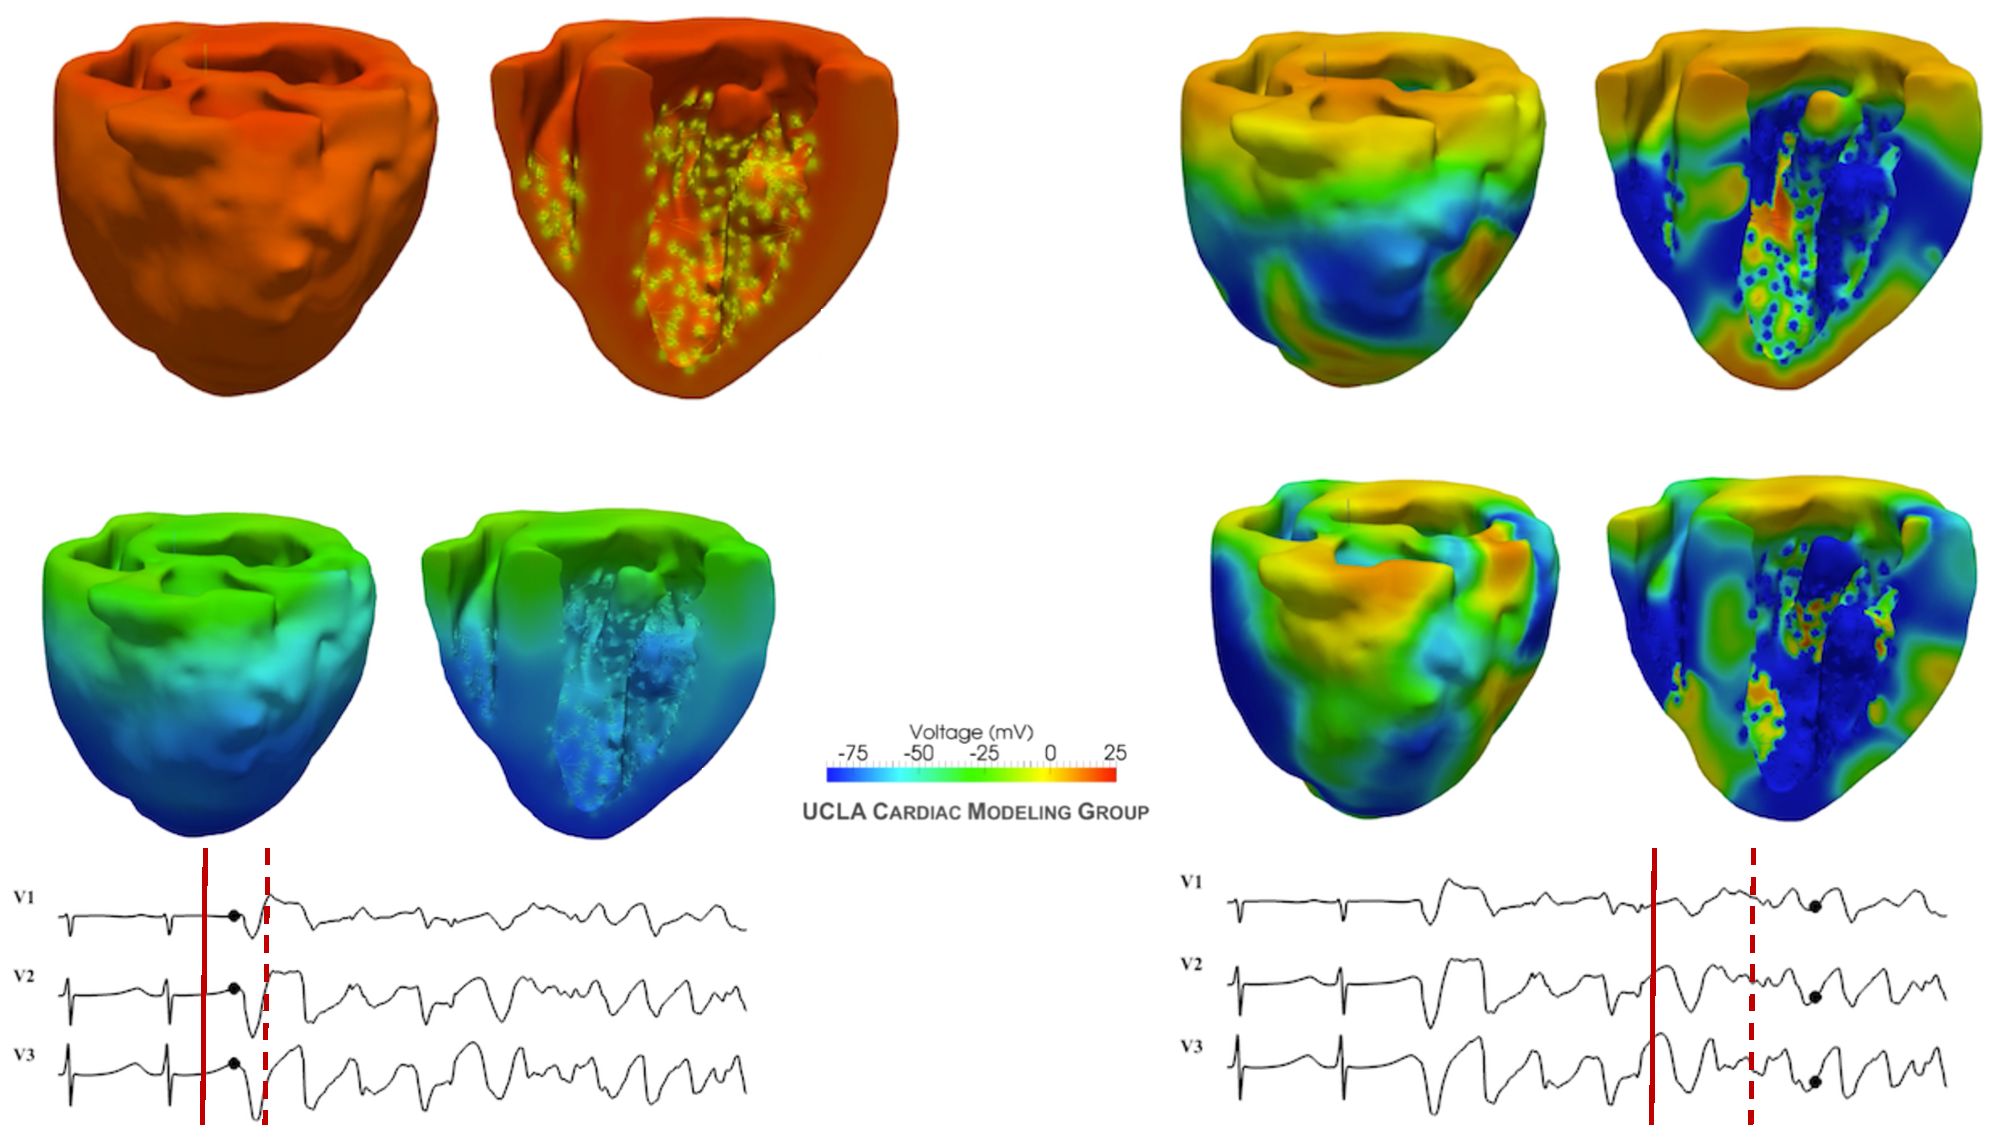
\includegraphics[width=0.9\linewidth]{figures/whnsrvfLowres.pdf}
%	\caption{Electrical activity during NSR and VF. The 
%	color scale runs from blue = rest state to red = excited (aka 
%	depolarized) state. (Colors in digital version).
%		In the top left, the ventricles are shown from two different 
%		angles, during a phase of NSR. The ventricles are fully 
%		exicted. The bottom left panel shows a later phase of the 
%		same beat, where the ventricles are progressively relaxing, 
%		starting with the apex (the pointed tip of the heart). This 
%		orderly propagation insures adequate muscle contraction and 
%		blood flow.
%		Three surface ECGs are shown beneath the left column, with 
%		red bars indicating the timing of the two snapshots. Note the 
%		periodic pattern.
%		The right column shows two snapshots during VF (earlier 
%		snapshot on top).
%		Note the disorganized nature of the electrical activity, 
%		wavefront breakup, and the multiple regions of 
%		depolarization. Note also the change in the surface ECG from 
%		periodic and regular (early on) to disorganized.
%		The AMA reads two such signals (obtained, however, 
%		intra-cardially and not from the surface) and tries to detect 
%		fibrillation. [Obtained from video of a simulation of the 
%		ventricles by the UCLA Cardiac Modeling Group, courtesy of 
%		Luigi Perrotti]}
%	\label{fig:whnsrvf}
%\end{figure*}